\chapter{Anforderungen}
\label{sec:anford}

Die Anforderungen an das System seien im Use-Case-Diagramm aus Abbildung \ref{fig:analysehs} aufgef�hrt.

\begin{figure}[h]
  \centering
  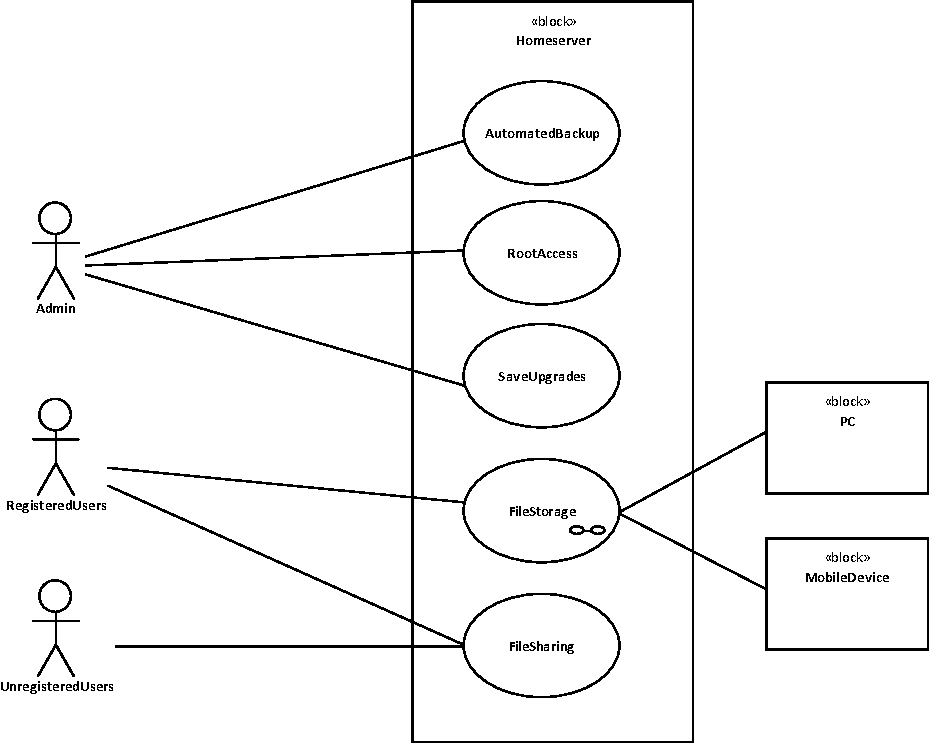
\includegraphics[scale=1]{anford/figures/AnalyseHS}
  \caption[Use-Case-Diagramm Homeserver]{Use-Case-Diagramm der Anforderungen an das System ,,Homeserver'' gegen�ber regestrierten und nicht registrierten Benutzern, sowie dem Administrator und der potentiell einsetzbaren Ger�te}
  \label{fig:analysehs}
\end{figure}

Besonders der Use-Case ,,SaveUpgrade'' war bei der Durchf�hrung des Projektes ein besonderer Schwerpunkt. Die Containervirtualisierung mit Docker erf�llt diese Anforderung. Der Anwendungsfall ,,FileStorage'' l�sst sich noch weiter verfeinern. Das separate Diagramm ist in Abbildung \ref{fig:analysefs} zu finden.

\begin{figure}[h]
  \centering
  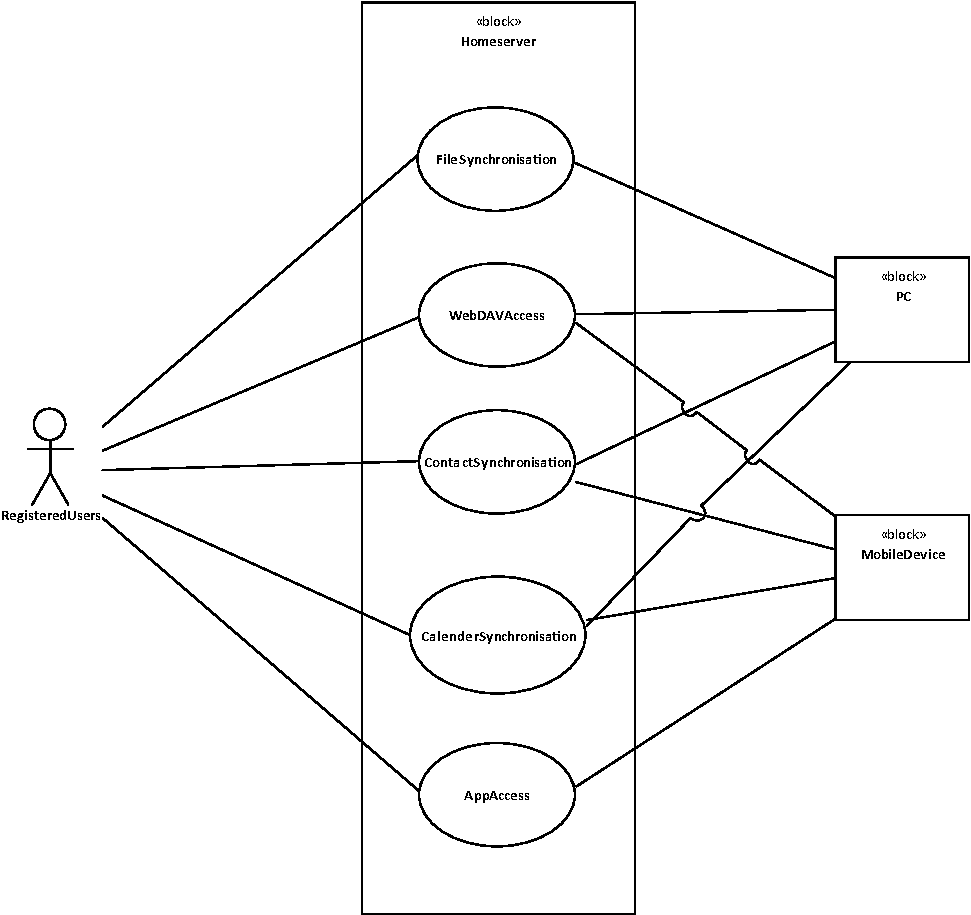
\includegraphics[scale=1]{anford/figures/AnalyseFS}
  \caption[Use-Case-Diagramm File Storage]{Verfeinerung des Anwendungsfalles ,,FileStorage''}
  \label{fig:analysefs}
\end{figure}


%%% Local Variables:
%%% mode: latex
%%% TeX-master: "../doku_server"
%%% End:
